\chapter{Knowledge}
\label{cha:knowledgei}

\section{Prerequisites}
This section will introduce some important knowledges, including sigmoid function, Bayes Formula, Huffman code, etc.

\subsection{Sigmoid Function}
Sigmoid function is a common kind of active function, the definition is
$$ \sigma(x) = \frac{1}{1+e^{-x}}, $$
The domain is $(-\infty, \infty)$, the range is $(0,1)$. And Figure~\ref{fig:sigmoid} shows the sigmoid function.
\begin{figure}[!ht]
  \centering
	\fbox{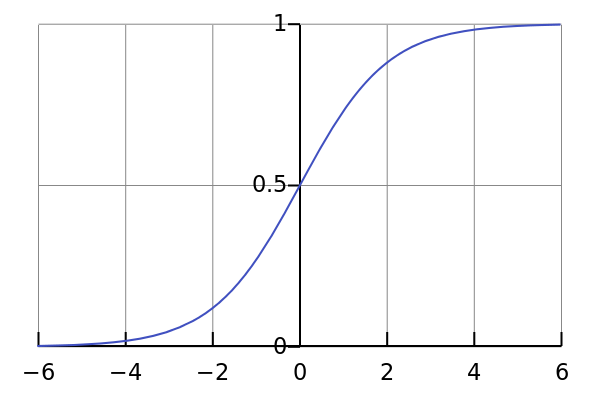
\includegraphics[width=0.5\textwidth]{sigmoid} }
	\caption{Sigmoid Function}
	\label{fig:sigmoid}
\end{figure}

Sigmoid function has the \textbf{derivative function} as following:
$$ \sigma^\prime(x) = \sigma(x)[1-\sigma(x)], $$
Thus, the \textbf{derivative functions} of $\mathrm{log}\sigma(x)$ and $\mathrm{log}(1-\sigma(x))$ are respectively
\begin{equation} 
[\mathrm{log}\sigma(x)]^\prime = 1-\sigma(x), \ [\mathrm{log}(1-\sigma(x))]^\prime = -\sigma(x), 
\end{equation}
Equation (2.1) will be used later in the derivation.

\subsection{Logistic Regression}
Binary classification is a very common task, e.g. , if an email is spam, if a customer is a potential customer, if a online transaction fraud, etc. Let ${\{(\mathbf{x}_i,y_i)\}}^m_{i=1}$ be the sample data of a binary classification problem, where $\mathbf{x}_i \in \mathbb{R}^n$, $y_i \in \{0,1\}$, when $y_i = 1$ the corresponding sample is $\mathbf{positive}$, when $y_i = 0$ the corresponding sample is $\mathbf{negative}$.

As for some sample data $\mathbf{x} = (x_1,x_2,\cdots,x_n)^T$, the hypothesis function can be written as
$$h_\theta(\mathbf{x}) = \sigma(\theta_0+\theta_1 x_1+\theta_2 x_2+\cdots+\theta_n x_n),$$
where $\theta = (\theta_0,\theta_1,\cdots,\theta_n)^T$ is the undetermined parameter. To simplify the formula, introduce $x_0 = 1$, and then $\mathbf{x}$ is extended to $(x_0,x_1,x_2,\cdots,x_n)^T$. Without confusing it is also recorded as $\mathbf{x}$. Thus, $h_0$ can be simplified as 
$$h_\theta(\mathbf{x}) = \sigma(\theta^T \mathbf{x}) = \frac{1}{1+e^{-\theta^T \mathbf{x}}}.$$

Let threshold $T = 0.5$, then the discriminant formula for binary classification is
$$y(\mathbf{x})=
\begin{cases}
1,& h_\theta(\mathbf{x})\geq 0.5;\\
0,& h_\theta(\mathbf{x})\le 0.5.
\end{cases}$$

How to calculate $\theta$ ? The usual method is, firstly determine a form of the \textbf{overall loss function} as following
$$ J(\theta) = \frac{1}{m}\sum^m_{i=1}cost(\mathbf{x}_i,y_i),$$
and then optimize it to obtain the optimal parameters $\theta^*$.

In practice, the loss function of a single sample $cost(\mathbf{x}_i,y_i)$ is often taken as the \textbf{log-likelihood function}
$$cost(\mathbf{x}_i,y_i)=
\begin{cases}
-\mathrm{log}(h_\theta(\mathbf{x}_i)),& y_i=1;\\
-\mathrm{log}(1-h_\theta(\mathbf{x}_i)),& y_i=0.
\end{cases}$$
Note that the above formula is a piecewise function, which can also be written in its overall expression as following
$$cost(\mathbf{x}_i,y_i) = -y_i\cdot\mathrm{log}(h_\theta(\mathbf{x}_i))-(1-y_i)\cdot(1-h_\theta(\mathbf{x}_i)).$$

\subsection{Bayes Formula}
Bayesian formula is put forward by the British mathematician Thomas Bayes, used to describe the relationship between two conditional probabilities. Let $P(A)$ and $P(B)$ respectively be the probability of event A and the probability of event B, $P(A|B)$ be the probability of the event A when event B occurs, and $P(A,B)$ be the probability of event A and B occurring simultaneously, so we have
$$P(A|B)=\frac{P(A,B)}{P(B)}, P(B|A)=\frac{P(A,B)}{P(A)}, $$
further, we can get
$$P(A|B)=P(A)\frac{P(B|A)}{P(B)},$$
this is the \textbf{Bayesian formula}.

\subsection{Huffman Coding}

\subsubsection{Huffman Tree}
In computer science, \textbf{tree} is a kind of nonlinear data structure, which is the structure of data elements (called \textbf{node} in the tree) organized in branch. The collection of several disjoint trees is called \textbf{forest}. The following are some common concepts about tree.
\begin{itemize}
\item \textbf{Path} and \textbf{Path Length}\\
In a tree, a path is a road from any node to its direct or indirect child. The number of branches is called path length of the path. If the provisions of the root layer No. 1, from the root node to the first node L layer path length L-1.
\item \textbf{Weighted Node} and \textbf{Weighted Path Length}\\
blabla..
\end{itemize}

\subsubsection{Huffman Tree Construction}

\subsubsection{Huffman Coding}

%--------------------------------------------------------------------------------------------------------------------------------%

\section{Skip-gram model}


